\subsection{Simulering af 2. ordens lavpasfilter}

\subsubsection{Simulering af 1 k$\Omega$ }
$\tau_5$ er via figur \ref{1k.stigetid} afmålt til 4.966 V, altså det tidspunkt, \\ hvor vores kurve er vokset med 5 $\tau$

Stigetiden bestemmes ved formlen:
\begin{center}
$t_{90} - t_{10} = stigetid$
\end{center}

Ud fra målinger af figur \ref{1k.stigetid} er stigetiden blevet beregnet til

\begin{center}
$t_{90} = 4.966 V \cdot 0.9 = 4.473 V$
\\ 
$t_{10} = 4.966 V \cdot 0.1 = 0.497 V$
\end{center}

Tidsforskellen mellem $t_{90}$ og $t_{10}$ måles via figur \ref{1k.stigetid} til 1.6 $\mu$s

\begin{figure}[h]
 \begin{center}
  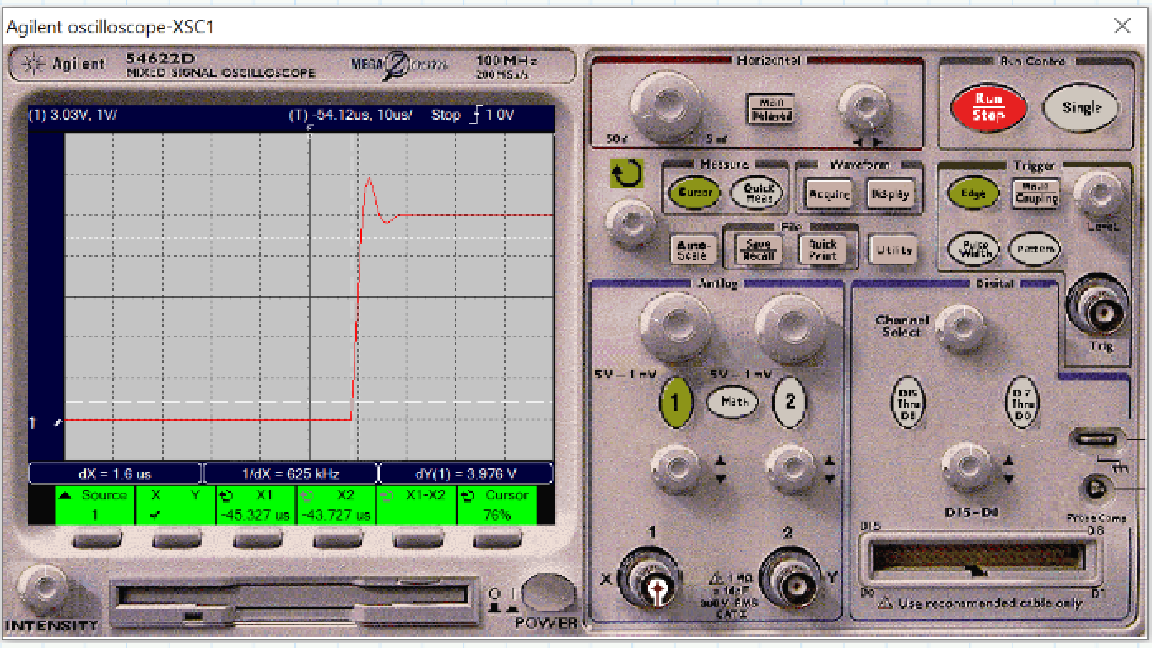
\includegraphics[height=5cm]{P_Fig/figur8_1k_stigetid}
  \caption{Stigetid}
  \label{1k.stigetid}
 \end{center}
\end{figure}

Maksimal spænding bestemmes ved formlen:
\begin{center}
$V_{max} - V_{min}$ = Maksimal spænding
\end{center}

Afstanden mellem $V_{max}$ og $V_{min}$ måles via figur \ref{1k_max} til 5.876 V

\begin{figure}[h]
 \begin{center}
  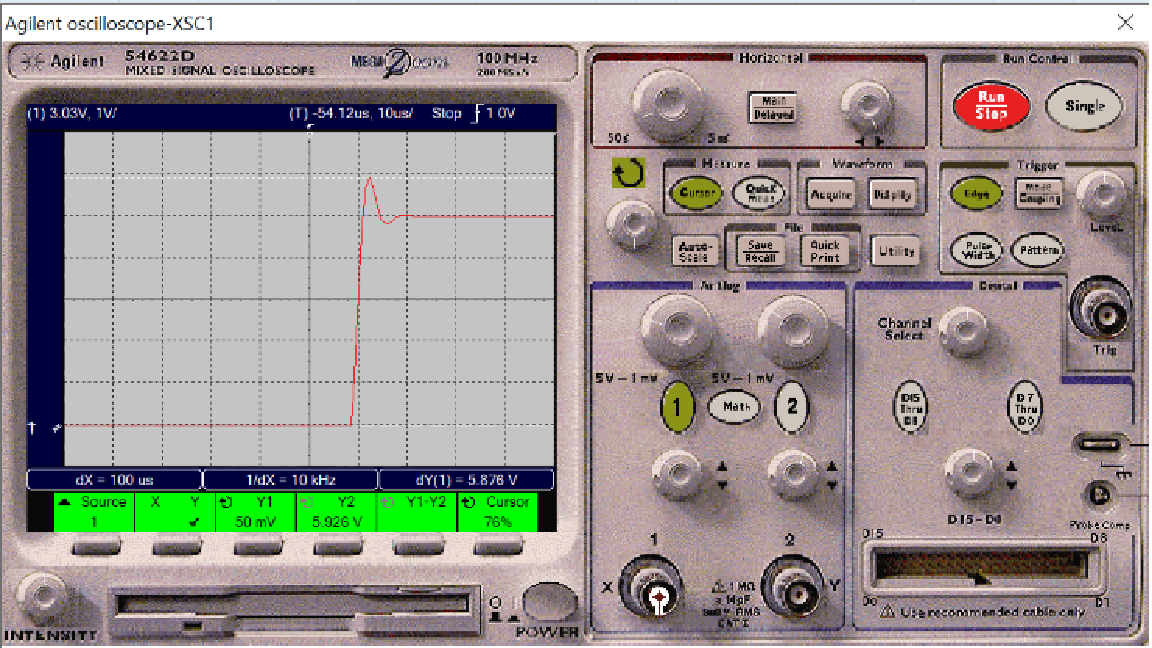
\includegraphics[height=5cm]{P_Fig/figur9_1k_max}
  \caption{Maksimal spænding}
  \label{1k_max}
 \end{center}
\end{figure}

\subsubsection{Simulering af 10 k$\Omega$ }
$\tau_5$ er via figur\ref{10k.stigetid} afmålt til 4.956 V, altså det tidspunkt, \\ hvor vores kurve er vokset med 5 $\tau$

Stigetiden bestemmes ved formlen:
\begin{center}
$t_{90} - t_{10} = stigetid$
\end{center}

Ud fra målinger af figur \ref{10k.stigetid} er stigetiden blevet beregnet til

\begin{center}
$t_{90} = 4.956 V \cdot 0.9 = 4.46 V$
\\ 
$t_{10} = 4.956 V \cdot 0.1 = 0.496 V$
\end{center}

Tidsforskellen mellem $t_{90}$ og $t_{10}$ måles via figur \ref{10k.stigetid} til 20.6 $\mu$s

\begin{figure}[h]
 \begin{center}
  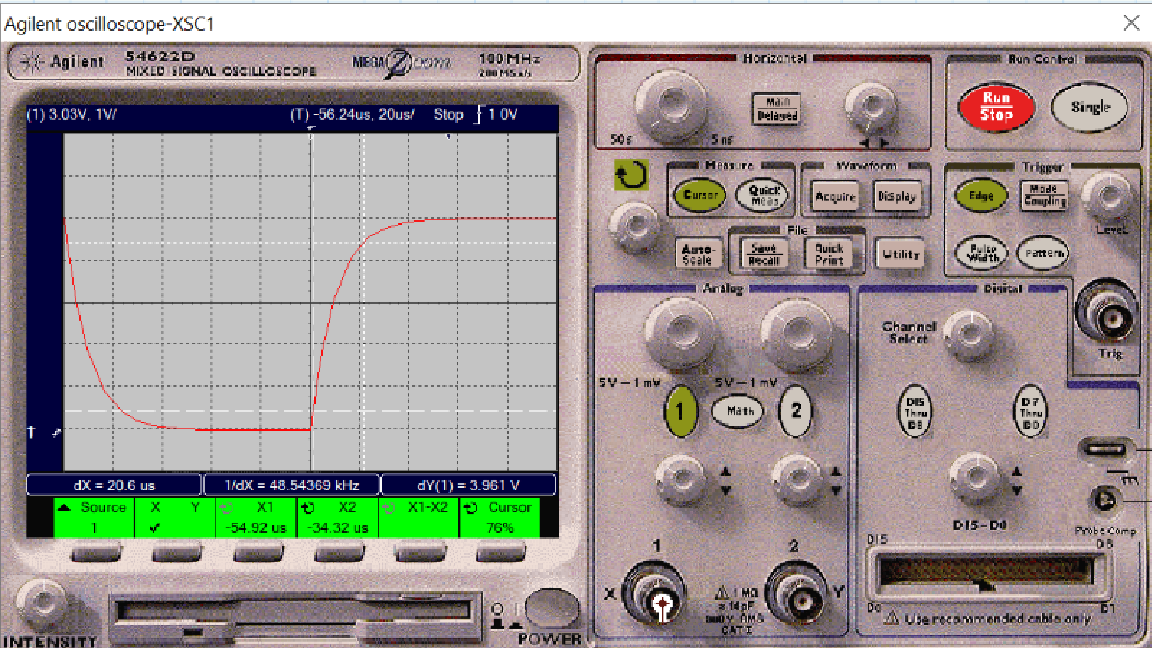
\includegraphics[height=5cm]{P_Fig/figur10_10k_stigetid}
  \caption{Stigetid}
  \label{10k.stigetid}
 \end{center}
\end{figure}

Maksimal spænding bestemmes ved formlen:
\begin{center}
$V_{max} - V_{min}$ = Maksimal spænding
\end{center}

Afstanden mellem $V_{max}$ og $V_{min}$ måles via figur \ref{10k_max} til 4.941 V

\begin{figure}[h]
 \begin{center}
  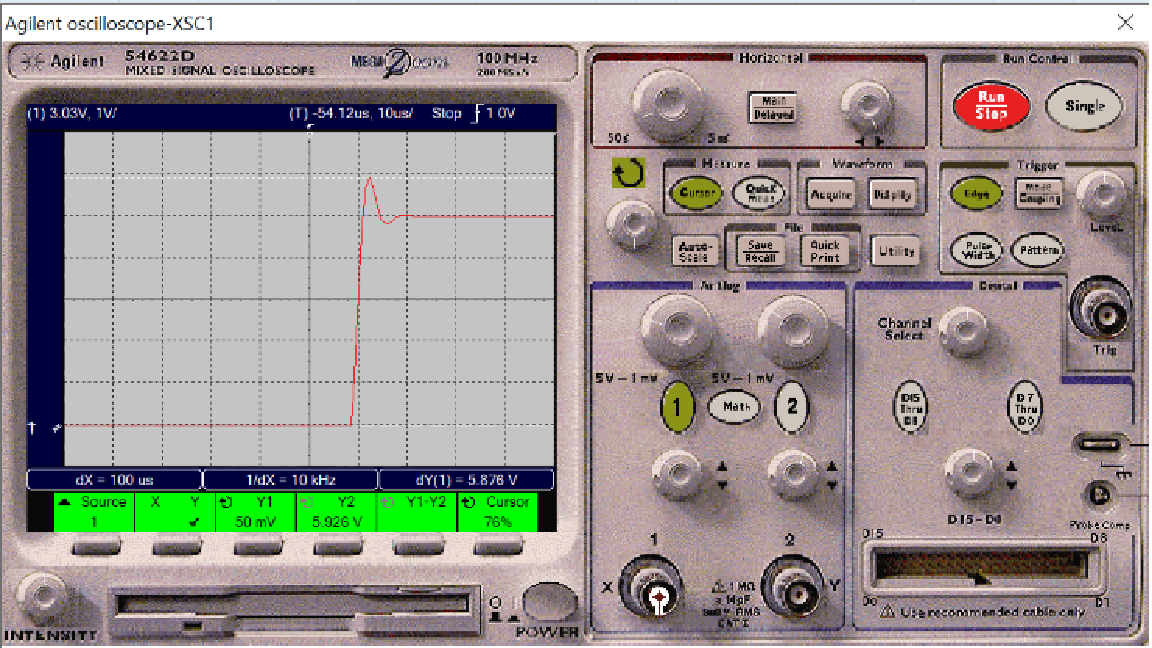
\includegraphics[height=5cm]{P_Fig/figur9_1k_max}
  \caption{Maksimal spænding}
  \label{10k_max}
 \end{center}
\end{figure}